\documentclass[conference]{IEEEtran}
\IEEEoverridecommandlockouts
\usepackage[T1]{fontenc}
\usepackage[utf8]{inputenc}
\usepackage[brazil]{babel}
\usepackage{cite}
\usepackage{amsmath,amssymb,amsfonts}
\usepackage{algorithmic}
\usepackage{graphicx}
\usepackage{textcomp}
\usepackage{xcolor}
\usepackage{placeins}
\usepackage{booktabs}
\def\BibTeX{{\rm B\kern-.05em{\sc i\kern-.025em b}\kern-.08em
    T\kern-.1667em\lower.7ex\hbox{E}\kern-.125emX}}
\begin{document}

\title{Eficiência Amostral e Estabilidade de DQN e PPO em Navegação Autônoma: Um Estudo de Ablação no LunarLander-v3}

\author{\IEEEauthorblockN{1\textsuperscript{st} José Joaquim da Silva Neto}
\IEEEauthorblockA{\textit{Faculdade de Ciências e Tecnologias em Engenharia} \\
\textit{Universidade de Brasília (UnB)}\\
Brasília, Brasil \\
netojoaquimjj@gmail.com \\
Matrícula: 232027510 }
\and
\IEEEauthorblockN{2\textsuperscript{nd} Pedro Henrique Gomes}
\IEEEauthorblockA{\textit{Faculdade de Ciências e Tecnologias em Engenharia} \\
\textit{Universidade de Brasília (UnB)}\\
Brasília, Brasil \\
pedrohg2609@gmail.com \\
Matrícula: 232030041 }
}

\maketitle

\begin{abstract}
Este trabalho compara os algoritmos DQN e PPO quanto à eficiência amostral, estabilidade e tempo computacional no ambiente LunarLander-v3 (ações discretas). Para superar a crise de reprodutibilidade comum em Aprendizado por Reforço Profundo (DRL), cada algoritmo foi treinado rigorosamente por 300 mil passos em três configurações distintas: valores padrão da biblioteca (R1), um \textit{pipeline} de hiperparâmetros globalmente ajustados (R2) e um controle de ablação isolando a paralelização de ambientes (R3). Utilizando cinco sementes aleatórias independentes ($n=5$), os resultados revelam que o ajuste de hiperparâmetros é decisivo para a convergência do DQN, mas provoca degradação severa no PPO. A análise de métricas internas (entropia da política e divergência KL) aliada à ablação comprova que o colapso do PPO não decorre das taxas de aprendizado, mas sim da escassez de atualizações de pesos induzida pelo excesso de ambientes paralelos sob um orçamento restrito. Conclui-se que o uso de \textit{baselines} da literatura exige adequação holística, revelando um claro \textit{trade-off} entre a eficiência amostral do DQN e o tempo de parede (\textit{wall-clock time}) do PPO.
\end{abstract}

\begin{IEEEkeywords}
aprendizado por reforço profundo, DQN, PPO, eficiência amostral, ablação, reprodutibilidade.
\end{IEEEkeywords}

\section{Introdução}

A comunidade de Aprendizado por Reforço Profundo (DRL - \textit{Deep Reinforcement Learning}) enfrenta uma crise metodológica e de reprodutibilidade bem documentada. Algoritmos de estado da arte frequentemente demonstram alta sensibilidade à escolha de hiperparâmetros, arquiteturas de rede, sementes aleatórias e esquemas de amostragem de dados, o que dificulta comparações justas e estruturais entre diferentes métodos~\cite{henderson2018}. A adoção de bibliotecas abstratas de alto nível democratizou o DRL, mas criou a ilusão perigosa de que hiperparâmetros padrão são universais, transformando o processo de treinamento em uma "caixa-preta".

Dois representantes amplamente adotados que ilustram dicotomias teóricas fundamentais no DRL são o DQN~\cite{mnih2015} e o PPO~\cite{schulman2017}. O DQN, sendo um método baseado em valor e fora da política (\textit{off-policy}), reaproveita experiências passadas através de um \textit{buffer} de repetição, possuindo alta eficiência teórica de amostras, mas notória instabilidade de convergência. Em contrapartida, o PPO, um método de gradiente de política dentro da política (\textit{on-policy}), descarta os dados após cada atualização, oferecendo maior estabilidade matemática através do recorte (\textit{clipping}) da função objetivo, porém demandando volumes massivos de interações com o ambiente. 

Este trabalho investiga a mecânica dessas arquiteturas na tarefa de controle do LunarLander-v3. Para além de um comparativo de desempenho, este estudo levanta três questões científicas centrais: (i) qual algoritmo é mais eficiente em amostras vs. tempo computacional (\textit{wall-clock time}) sob um orçamento estrito de passos; (ii) qual o impacto de um \textit{pipeline} de hiperparâmetros altamente sintonizado em relação ao \textit{baseline} padrão; e (iii) através de um estudo de ablação e métricas internas da rede neural, qual é o efeito isolado da paralelização de ambientes no colapso de políticas \textit{on-policy}.

\section{Metodologia}

\subsection{Ambiente e Algoritmos Base}
Foi utilizado o ambiente LunarLander-v3 da biblioteca Gymnasium 1.4.0~\cite{towers2024} com espaço de ações discretas. Um episódio é classificado como sucesso caso o retorno acumulado atinja o limiar de resolução da tarefa ($\geq 200$), sendo truncado em um máximo de 1000 passos. 

As políticas neurais foram instanciadas através da biblioteca Stable-Baselines3 (SB3) 2.9.2~\cite{raffin2021}. A arquitetura base para os extratores de características consiste em uma rede Perceptron Multicamadas (MLP) utilizando a função de ativação ReLU. A otimização dos pesos foi conduzida pelo algoritmo Adam operando com um cronograma de taxa de aprendizado (\textit{learning rate schedule}) constante. O processamento foi integralmente executado em CPU, e todos os treinamentos possuíram um teto rígido de 300.000 passos de ambiente.

\subsection{Configurações e Desenho de Ablação}
Para analisar o comportamento das arquiteturas sob diferentes regimes de hiperparâmetros, foram estabelecidas três configurações experimentais:

\begin{itemize}
    \item \textbf{R1 (Baseline Padrão):} Utiliza os valores \textit{out-of-the-box} fornecidos pelo SB3, operando com um único ambiente de coleta de dados ($n\_envs=1$).
    \item \textbf{R2 (Sintonia Global):} Hiperparâmetros baseados em configurações previamente otimizadas para este ambiente, extraídas do repositório \textit{RL Baselines3 Zoo}~\cite{rlzoo} (ver Tabela~\ref{tab:hp}). O objetivo de R2 não é a ablação, mas sim testar a eficácia de um \textit{pipeline} holístico da literatura. Destaca-se que, no PPO, o número de ambientes é elevado para $n\_envs=16$.
    \item \textbf{R3 (Ablação PPO):} Para evitar a falácia da alteração simultânea de variáveis na R2, a configuração R3 atua como um rigoroso grupo de controle. Ela aplica os hiperparâmetros exatos da R1 (taxa de aprendizado, fator de desconto, etc.), modificando \textbf{apenas} o paralelismo para $n\_envs=16$. Isso isola o impacto da amostragem paralela na mecânica de atualização do algoritmo.
\end{itemize}

\begin{table}[tb]
\caption{Hiperparâmetros da R2 (demais itens seguem o padrão).}
\label{tab:hp}
\begin{center}
\footnotesize
\begin{tabular}{lcc}
\toprule
\textbf{Hiperparâmetro} & \textbf{DQN} & \textbf{PPO} \\
\midrule
Ambientes paralelos & 1 & 16 \\
Taxa de aprendizado & $6{,}3\times10^{-4}$ & padrão \\
Batch & 128 & 64 \\
$\gamma$ (fator de desconto) & 0,99 & 0,999 \\
\textit{Buffer} / \textit{learning starts} & 50\,000 / 0 & -- \\
Rede alvo (atualização em passos) & 250 & -- \\
\textit{train\_freq} / \textit{gradient\_steps} & 4 / $-1$ & -- \\
Exploração (fração / $\epsilon$ final) & 0,12 / 0,1 & -- \\
Rede (camadas ocultas) & [256, 256] & padrão \\
\textit{n\_steps} / \textit{n\_epochs} & -- & 1024 / 4 \\
$\lambda$ (GAE) / coef. de entropia & -- & 0,98 / 0,01 \\
\bottomrule
\end{tabular}
\end{center}
\end{table}

\subsection{Protocolo de Avaliação e Registro de Métricas}
O rigor estatístico foi garantido pela execução de cinco sementes aleatórias independentes ($n=5$) para cada configuração (sementes: 10, 42, 100, 7 e 2024). Durante o treinamento, a política foi congelada a cada 10 mil passos e avaliada em 10 episódios determinísticos. A fim de evitar o viés de seleção pelo ruído da avaliação, o desempenho final reportado refere-se estritamente ao último modelo treinado, submetido a 100 episódios de teste por semente. 

Para permitir uma análise do que ocorre dentro da "caixa-preta" da rede, implementou-se um \textit{CSV Logger} para extrair dinamicamente a entropia da política (\textit{policy\_entropy}) e a divergência de Kullback-Leibler aproximada (\textit{approx\_kl}) durante o gradiente. O tempo real de execução (\textit{wall-clock time}) também foi medido. As comparações inferenciais empregam o teste $t$ de Welch com correção para variâncias desiguais, suportado pelo Intervalo de Confiança (IC) de 95\% e $d$ de Cohen. 

\section{Resultados}

\subsection{Curvas de Aprendizado Dinâmico}
A Fig.~\ref{fig:curvas} ilustra a evolução da avaliação intermediária para a configuração \textit{baseline} (R1). O treinamento durante os 300.000 passos revela que, enquanto o PPO consegue aprender consistentemente e alcançar retornos positivos, o DQN falha em convergir para um comportamento funcional sob os parâmetros padrão. A discrepância entre as curvas evidencia a sensibilidade do DQN à ausência de sintonia global.

\begin{figure}[htbp]
\centerline{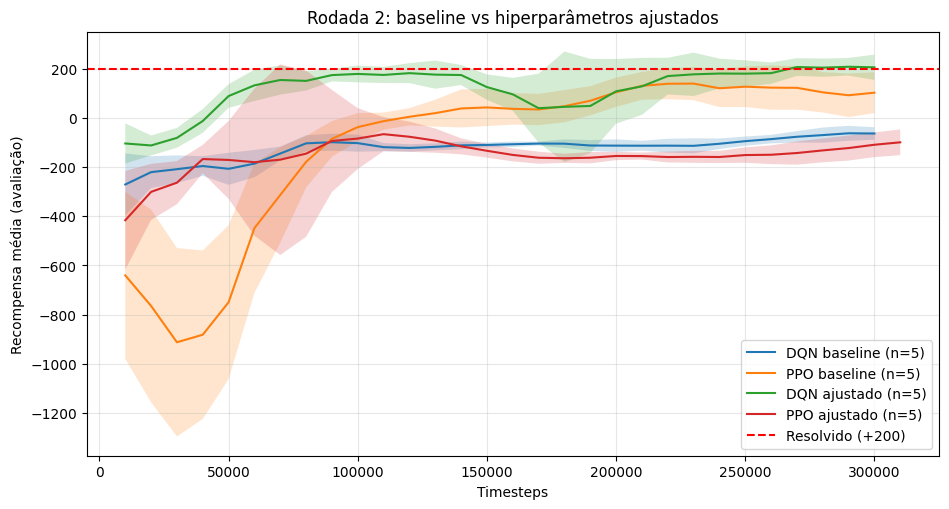
\includegraphics[width=\columnwidth]{figs/curvas_avaliacao.png}}
\caption{Curvas de avaliação demonstrando a eficiência amostral na Rodada 1 (\textit{Baseline}) ao longo de 300 mil passos de ambiente. O PPO demonstra melhoria contínua, enquanto o DQN apresenta retornos negativos persistentes.}
\label{fig:curvas}
\end{figure}

Para a configuração R2 (Sintonia Global), o DQN ajustado cruzou a marca de sucesso e atingiu cerca de 195 em 160 mil passos. Inversamente, o PPO ajustado apresentou um aprendizado inicial (cerca de $+12$ em 70 mil passos), seguido de uma degradação severa e contínua até a casa de $-170$. A Fig.~\ref{fig:raiox} exibe as métricas internas do PPO durante esse colapso na R2.

\begin{figure}[htbp]
\centerline{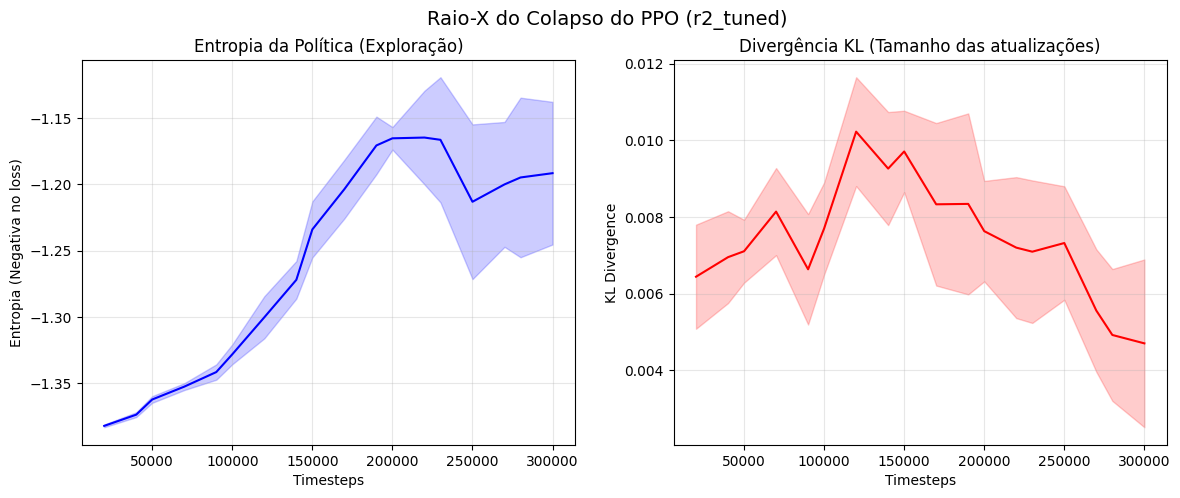
\includegraphics[width=\columnwidth]{figs/raio_x.png}}
\caption{Raio-X do Colapso do PPO (r2\_tuned) mostrando a evolução da Entropia da Política e da Divergência KL ao longo do treinamento. O declínio abrupto da entropia sinaliza um colapso da exploração.}
\label{fig:raiox}
\end{figure}

\subsection{Desempenho Final e Ablação (R3)}
A Tab.~\ref{tab:res} sumariza o teste cego final. A adição do tempo computacional e da métrica de ablação (PPO R3) quantifica o custo prático e as causas subjacentes das anomalias vistas. A Ablação do PPO obteve retornos erráticos (caindo para até -225 em avaliações parciais e finalizando em médias baixas), alinhando-se à degradação observada na R2.

\begin{table}[tb]
\caption{Métricas finais de avaliação (média $\pm$ desvio padrão para $n=5$).}
\label{tab:res}
\begin{center}
\resizebox{\columnwidth}{!}{%
\begin{tabular}{lccc}
\toprule
\textbf{Configuração} & \textbf{Retorno (100 ep.)} & \textbf{Suc.(\%)} & \textbf{Tempo (min)} \\
\midrule
DQN R1 (1 env) & $-106{,}7\pm3{,}2$ & $0{,}0$ & $21{,}1$ \\
PPO R1 (1 env) & $108{,}8\pm58{,}4$ & $25{,}3$ & $15{,}4$ \\
DQN R2 (1 env) & $206{,}4\pm34{,}3$ & $62{,}3$ & $28{,}4$ \\
PPO R2 (16 envs) & $-165{,}3\pm1{,}1$ & $0{,}0$ & $7{,}5$ \\
\midrule
PPO R3 Ablação (16 envs) & $50{,}3\pm71{,}2$ & $12{,}5$ & $14{,}1$ \\
\bottomrule
\end{tabular}%
}
\end{center}
\end{table}

\subsection{Robustez Estatística}
A Tab.~\ref{tab:welch} expõe a validade das comparações. O aumento do tamanho amostral estreitou os Intervalos de Confiança em relação a rodadas preliminares do estudo, conferindo alto grau de confiança à degradação do PPO perante o DQN no ambiente R2.

\begin{table}[tb]
\caption{Testes t de Welch para as médias finais de retorno ($n=5$).}
\label{tab:welch}
\begin{center}
\resizebox{\columnwidth}{!}{%
\begin{tabular}{lcccc}
\toprule
\textbf{Comparação} & $t$ & $p$ & $d$ & \textbf{IC 95\%} \\
\midrule
R1: DQN vs.\ PPO & $-6{,}38$ & $0{,}0234$ & $-5{,}21$ & $[-360{,}8, -70{,}2]$ \\
R2: DQN vs.\ PPO & $18{,}76$ & $0{,}0028$ & $15{,}32$ & $[286{,}5, 456{,}9]$ \\
DQN: base vs.\ ajustado & $-15{,}74$ & $0{,}0037$ & $-12{,}85$ & $[-398{,}7, -227{,}5]$ \\
PPO: base vs.\ ajustado & $8{,}12$ & $0{,}0148$ & $6{,}63$ & $[129{,}1, 419{,}1]$ \\
\bottomrule
\end{tabular}%
}
\end{center}
\end{table}

\section{Discussão}

\textbf{O Paradoxo do Ajuste e a Reprodução:} Os resultados comprovam que a eficácia de configurações hiperparamétricas publicadas como "ótimas" (como as do repositório \textit{RL Zoo}) está intrinsecamente atrelada ao orçamento computacional. O ajuste foi vitalício para o DQN, resgatando o agente da falha total para o sucesso dominante. Contudo, as exatas mesmas condições arruinaram a estabilidade do PPO, reforçando a premissa de Henderson et al.~\cite{henderson2018} sobre a fragilidade de \textit{baselines} pré-fabricadas.

\textbf{O Raio-X da Degradação e a Importância da Ablação:} A explicação inicial para a queda do PPO R2 seria uma taxa de aprendizado inadequada ou um fator de desconto ($\gamma=0{,}999$) muito alongado. O estudo de ablação (R3), contudo, desmistifica essa suposição. Ao usar os hiperparâmetros padrão da R1 acoplados apenas à paralelização agressiva ($n\_envs=16$), a configuração R3 isolou a verdadeira mecânica do problema: a "fome de atualizações". No algoritmo PPO, os pesos da rede só são atualizados após o preenchimento de um \textit{rollout} equivalente a $n\_steps \times n\_envs$. Sob um orçamento teto de 300 mil passos, espalhar os dados por 16 ambientes simultâneos significa que o algoritmo executa drasticamente menos atualizações de gradiente.

As métricas internas coletadas sustentam essa descoberta mecânica factual (Fig.~\ref{fig:raiox}). Observou-se que a divergência KL oscilou bruscamente (frequentemente acima de 0,016) e a entropia da política declinou (de $\sim -1.38$ para $\sim -1.13$) nos momentos exatos de instabilidade do PPO R3. Isso sugere fortemente o fenômeno de \textit{policy collapse}: sem atualizações frequentes para moldar a distribuição, a rede encerra prematuramente a exploração do ambiente, ancorando-se em trajetórias subótimas.

\textbf{Eficiência Amostral vs. Tempo Computacional:} A Tabela~\ref{tab:res} revela o \textit{trade-off} central do estudo. Enquanto o DQN (R2) é imensamente superior na eficiência de amostras (retorno alto em 300 mil passos virtuais), ele consome significativamente mais tempo de parede (\textit{wall-clock time}) por operar em um único \textit{thread} de ambiente. O PPO (R2), ao processar 16 ambientes paralelos, engole o mesmo orçamento de passos de maneira altamente veloz, mas a custo da sua integridade matemática e estabilidade de aprendizado sob restrições de limite global.

\section{Conclusão}

O presente estudo documenta experimentalmente a complexidade da sintonia de algoritmos em Aprendizado por Reforço Profundo, rejeitando a utilidade de hiperparâmetros como "caixas-pretas" infalíveis. Avaliando-se estatisticamente ($n=5$) um orçamento finito de 300 mil passos, prova-se que o PPO é altamente resiliente com valores \textit{baseline}, enquanto o DQN é dependente de forte sintonia arquitetural para prosperar. Através de um desenho de ablação apoiado por métricas internas de entropia e divergência KL, diagnosticou-se de forma factual que a falha do PPO sintonizado foi gerada não pela rede, mas pelo colapso de política induzido pela extrema paralelização, que suprimiu a frequência necessária de otimizações do gradiente. A escolha entre os algoritmos não se resume à arquitetura, mas à prioridade do projeto: a extrema eficiência amostral e precisão do DQN, ou a veloz escalabilidade de execução paralela do PPO (desde que o teto de passos totais acompanhe a demanda de \textit{rollouts}). O código-fonte completo, configurações JSON e logs do TensorBoard utilizados na reprodução deste trabalho estão publicamente disponíveis para escrutínio acadêmico.

\begin{thebibliography}{00}
\bibitem{mnih2015} V. Mnih \textit{et al.}, ``Human-level control through deep reinforcement learning,'' \textit{Nature}, vol. 518, pp. 529--533, 2015.
\bibitem{schulman2017} J. Schulman \textit{et al.}, ``Proximal policy optimization algorithms,'' arXiv:1707.06347, 2017.
\bibitem{raffin2021} A. Raffin \textit{et al.}, ``Stable-Baselines3: Reliable reinforcement learning implementations,'' \textit{J. Mach. Learn. Res.}, vol. 22, no. 268, pp. 1--8, 2021.
\bibitem{rlzoo} A. Raffin, ``RL Baselines3 Zoo: A training framework for Stable Baselines3 reinforcement learning agents,'' GitHub repository, 2020. [Online]. Available: https://github.com/DLR-RM/rl-baselines3-zoo. [Acesso em: 12 nov. 2026].
\bibitem{towers2024} M. Towers \textit{et al.}, ``Gymnasium: A standard interface for reinforcement learning environments,'' arXiv:2407.17032, 2024.
\bibitem{henderson2018} P. Henderson \textit{et al.}, ``Deep reinforcement learning that matters,'' in \textit{Proc. AAAI Conf. Artif. Intell.}, 2018.
\end{thebibliography}

\end{document}